\chapter{10 Questions with a Millionaire: Robert Miller on Cash Flow, Scarcity, and Compounding Skill}

This chapter follows a sequence that is tighter than it first appears. We begin with a teaser about personal brand and business durability, rewind into Robert Miller's early path through college, crypto, and digital marketing, and then move through a compact theory of scaling, a set of books for thinking at a higher level, a practical account of failure and partnership design, a speculative but revealing discussion of crypto and value, and finally a contrast between destructive borrowing and compounding self-investment. There is no blackboard mathematics in this interview, but there is a genuine quantitative spine, and it is useful to write that spine down carefully.

\begin{remark}
The displayed equations in this chapter are not recovered from a board. They are compact notations for structures that the speaker states verbally: the distinction between capital gains and cash flow, the pipeline from attention to revenue, the rule of thumb for partnerships, the heuristic relation between scarcity and energy cost, and the update rule by which self-investment compounds into later capability.
\end{remark}

\section{A Prologue on Reputation}

The lecture opens with the effect before the mechanism. Robert says that he built a personal brand alongside his first company, had to shut that company down, then repeated the process with a second agency, and was nevertheless able to scale the third business to multiple seven figures within roughly six months because the brand survived the collapse of the earlier vehicles. He adds that the same accumulated reputation helped launch a later business to a seven-figure runway within about sixty days.

Only after this preview do we get the formal reset: the interviewer introduces the series, introduces Robert Miller as an entrepreneur, investor, and multimillionaire, and asks for a quick background. That ordering matters. The teaser is not yet the argument; it is the payoff that the rest of the chapter has to explain.

What is already visible here is a distinction between a business mechanism and a durable commercial identity. Markets change, offers change, companies fail, partnerships unwind, but a recognized name in a market can carry information forward. In the remainder of the lecture, this claim will be rebuilt step by step: first through education and cash flow, then through scaling, then through failure, and finally through a broader account of money, learning, and motivation.

\section{From School to Cash Flow}

Robert's formal background begins in business administration and economics, but he quickly describes the mismatch: the school system did not fit the career path he was discovering for himself. The turning point came not from the degree program itself, but from an outside digital-marketing course. At the same time, he had already made money in crypto. The crucial thing, however, is that he does not count this as business success in the strong sense. He draws a clean line between gains from asset appreciation and the recurring output of a real operating business.

\paragraph{A first distinction.}
The lecture makes the following separation explicit:
\begin{equation}
CG \neq CF
\end{equation}
where \(CG\) denotes capital gains and \(CF\) denotes cash flow. A useful bookkeeping compression is
\begin{equation}
\Delta W = CG + CF,
\end{equation}
but the point of the lecture is not merely accounting. The point is strategic: one may enjoy a rise in wealth without yet having built a machine that produces ongoing inflow.

This distinction explains why the next move in the story is so important. Crypto had already produced money, but not structure. That is why Robert says he then needed to learn how to build cash flow and how to build a real business. From there his argument about college becomes narrower and more precise than a generic dismissal of school. For professions that require pedigree, such as doctors or lawyers, formal credentials remain necessary. But for entrepreneurship, the operative test is different: one must solve problems and construct a machine that brings in revenue.

We should keep the rhythm of this transition intact. It is not merely ``college versus no college.'' It is a shift from passive appreciation to active commercial architecture.

\section{Scaling Logic: Marketing, Sales, and Finance}

Once the lecture has moved from biography to method, Robert gives a remarkably compressed scaling model. First one must master marketing and bring in more revenue. But this is not merely a matter of paying for ads. He emphasizes content, traffic strategy, and the practical problem of getting people to care. From there one needs sales, because leads without the ability to convert them remain inert. Finally, one needs finance, not as an ornament at the end, but as the discipline that tells us how the cash actually moves.

\begin{figure}[h]
\centering
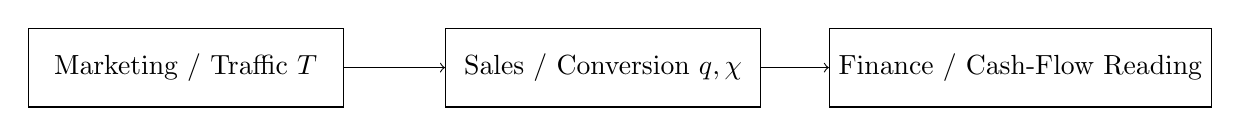
\begin{tikzpicture}
\node[draw, rectangle, minimum width=4cm, minimum height=1cm] (m) at (0,0) {Marketing / Traffic \(T\)};
\node[draw, rectangle, minimum width=4cm, minimum height=1cm] (s) at (5.3,0) {Sales / Conversion \(q,\chi\)};
\node[draw, rectangle, minimum width=4cm, minimum height=1cm] (f) at (10.6,0) {Finance / Cash-Flow Reading};
\draw[->] (m) -- (s);
\draw[->] (s) -- (f);
\end{tikzpicture}
\caption{An editorial compression of the scaling sequence stated in the interview: marketing creates attention, sales converts attention into revenue, and finance determines whether revenue becomes intelligible and usable cash flow.}
\end{figure}

If we write this sequence in a deliberately light symbolic form, we get
\begin{equation}
R \propto T \times q \times \chi,
\end{equation}
where \(R\) is revenue, \(T\) is traffic or attention, \(q\) is the fraction of that attention that becomes genuine opportunity, and \(\chi\) is sales effectiveness. Robert does not state this formula, but it is a faithful compression of the order in which he names the moving parts.

A natural next step is to compare one period with the next:
\begin{align}
\frac{R_{t+1}}{R_t}
   &\approx
   \frac{T_{t+1}}{T_t}
   \cdot
   \frac{q_{t+1}}{q_t}
   \cdot
   \frac{\chi_{t+1}}{\chi_t}.
\end{align}
This should be read only as a scaling heuristic. The lecture does not claim that business growth is literally multiplicative in this exact form. What it does claim is that growth usually requires improvement at several linked stages rather than a single tactical fix.

The finance step matters because high revenue is not yet the same thing as clean commercial control. We may have a revenue story that looks exciting from the outside and still lack usable cash flow, reliable payout timing, or an intelligible model of where the money is actually going. That is why finance arrives last in the spoken sequence, not because it is least important, but because it reads the consequences of the prior two stages.

\section{Books as an Operating System}

The interviewer next asks for the top three books everyone should read, and Robert answers in a sequence that is more architectural than inspirational. These are not offered as monuments to culture; they are assigned a function inside a business.

\begin{itemize}
\item \emph{The Road Less Stupid} is presented as the book that supplies mental frameworks: how to think ahead, how to think about what one is doing, and how not to remain trapped at the purely tactical level.
\item \emph{Multipliers} appears as a book for team construction: how to work with other people, multiply their efforts, and align interests.
\item \emph{Predictable Revenue} is presented as a book about how sales systems and sales teams are built to bring revenue in the door.
\end{itemize}

There is a clear motion here. First strategy, then team leverage, then organized revenue.

\subsection{Question \& Answer}

\paragraph{Question.}
What does it mean to move from tactics to frameworks?

\paragraph{Answer.}
In the language of the lecture, it means refusing to remain only the expert, the marketer, or the tactical operator. A framework is a way of seeing one step earlier and one level higher. It asks how an offer will roll out, who will be accountable, how a team will be held to the structure, and what one ought to be thinking about before the obvious problems arrive.

This is why Robert dwells on the first book as more than a recommendation. The point is not simply that a book contains useful ideas. The point is that business maturity requires a change in the level at which we think. Revenue tactics are necessary, but without a framework they tend to remain local optimizations. The lecture is beginning to push upward from action into architecture.

\section{Personal Brand, Failure, and the Geometry of Partnership}

The next section of the interview returns to the teaser, but now with explanation. Robert says that personal brand matters because the mechanism of what one does for people will change as markets change. A business may disappear, an offer may no longer fit, and yet the market's memory of a person can remain. That is the durable part.

He then recounts the sequence more fully. The first agency closed. The second agency also closed, in part because there were too many partners and the fit was wrong. Yet the third business scaled quickly because reputation and will had already been built in the marketplace around digital marketing and client acquisition. The argument is no longer a slogan. It is now tied to a concrete sequence of shutdown, survival, and relaunch.

The interviewer then pivots to failure, and Robert's answer tightens into a set of design constraints for partnership. The first is almost numerical:
\begin{equation}
N_p \lesssim 3.
\end{equation}
This is not a theorem, but it is very much stated as a rule of thumb. One does not need four or five partners in a company. Beyond a small number, the partnership can become unstable, diffuse, and harder to govern.

The rest of the partnership geometry is qualitative but exacting. A partner should bring something crucial to the business, whether connections, people, capital, execution, or network. A partner should not merely be likable. Values must align. Vision must align. There must be a real conversation about what each party brings to the table, where the business is going, and how each side will be called out when performance slips.

There is also a sharp demotion of ego in this section. Name, offer, even the claim ``I came up with this'' do not count for much unless the thing is executed. The lecture insists on a migration from symbolic ownership to operational responsibility. That is why this section follows the books section so naturally: once we have strategy, accountability becomes the next unavoidable subject.

\section{Cryptocurrency, Scarcity, and Energy Cost}

When the interviewer asks about cryptocurrency, the lecture changes register. We are no longer discussing only business technique. Robert presents crypto as ``not just a new tech,'' but as a new way of thinking about money. He immediately widens the frame beyond Bitcoin or Ethereum alone and brings in central banks, CBDCs, wealth storage, and the question of what society counts as valuable.

This section is the closest thing in the lecture to a conceptual argument of the sort we might want to formalize, but we should do so carefully. Robert is not presenting a settled economic theorem. He is staging a question.

\subsection{Question \& Answer}

\paragraph{Question.}
Is value grounded in rarity alone, or in scarcity backed by real cost?

\paragraph{Answer.}
Robert raises the contrast directly. Perhaps something is valuable simply because it is rare. Or perhaps value becomes more persuasive when real physical cost is tied to its creation or verification. Bitcoin enters here through mining and the physical electricity required to verify transactions. Gold enters through extraction and mining cost. The lecture does not finish the matter as a theorem; it offers the analogy as a way to think.

A concise heuristic notation for this is
\begin{equation}
V_{\text{asset}} \propto \sigma \times E_{\text{cost}},
\end{equation}
where \(\sigma\) denotes scarcity and \(E_{\text{cost}}\) denotes real extraction or verification cost. This is not Robert's formula; it is an editorial compression of his analogy.

We can write the spoken logic as a short derivation.
\begin{enumerate}
\item Ask whether value comes merely from rarity.
\item Ask whether value requires cost as well.
\item Observe that Bitcoin requires mining and energy to verify transactions.
\item Observe that gold requires mining and energy to extract.
\item Conclude that society may treat energy-backed scarcity differently from costless rarity.
\item Leave open the final practical question: do we transact with such an asset, or do we preserve wealth in it?
\end{enumerate}

The lecture also leaves the future deliberately unresolved. Robert asks what Web3.0 will look like and what a CBDC rollout will look like. He asks, in effect, what kind of money we are moving toward and what kind of human supervision may be built into that movement. The answer is not yet doctrinal. The lecture keeps the question alive.

\section{From First Windfall to Self-Investment}

After the abstract discussion of money, the interview narrows back down into chronology. Robert explains that he got into crypto around 2015--2016 after repeated conversations with someone deeply interested in that world. He mentions early Bitcoin at roughly \$800--\$1,000, Ethereum around \$17, and the AntShares-to-Neo transition as one of the projects on which he did especially well.

This is where the lecture provides its clearest numerical anecdote. Robert says that he put in roughly \$1.5k--\$2k and that within around four months this became roughly \$250k. If we turn that anecdote into a rough multiplicative example, we get
\begin{align}
I_0 &\approx \$1.5\text{k} \text{ to } \$2\text{k},\\
V_{4m} &\approx \$250\text{k},\\
M &= \frac{V_{4m}}{I_0} \approx 125\text{--}167.
\end{align}
This is not a valuation model. It is simply a way of preserving the scale of the reported transformation. The emotional force of the lecture at this moment lies precisely in that scale: a young college student sees a small speculative position turn into something enormous, and the result is not only amazement but a desire to explain the phenomenon to other people. He starts creating books and courses and speaking on stages. Teaching becomes part of the entrepreneurial form.

The interview then moves into a contrast between the worst and best financial decisions he made. The worst one is revealing because it is not described as a bad trade. It is described as a short-term borrowing episode used to cover payroll when payment processors were holding funds and the firm's cash mechanics were under stress. What made the decision bad was not just the debt; it was the asymmetry. He took the risk, and others in the company did not meaningfully share it. The financial mistake exposed the partnership structure.

The best decision, by contrast, was to invest the crypto gains into courses and later into mentorships. Robert says he spent roughly \$30k--\$40k on courses and broadened his understanding of stocks, e-commerce, and marketing. The point is not that one should become an expert in everything. The point is that one can accumulate a stock of capability that later makes revenue easier to generate.

A useful update rule for this part of the lecture is
\begin{align}
K_{t+1} &= K_t + \Delta K(I_t),\\
R_{t+1} &= R\bigl(K_{t+1}\bigr),
\end{align}
where \(K_t\) is the skill stock at time \(t\) and \(I_t\) is self-investment in courses, mentorships, and high-exposure environments. Again, this is editorial notation, not quoted mathematics. But it captures the lecture's causal claim: better skill produces better traction, and better traction makes later learning investments more potent.

The striking twist is that the ``last mastermind'' or the last mentorship may look like the catalyst only because earlier layers were already in place. The final connection matters because the previous ones were not wasted. This gives the lecture a very particular theory of compounding. It is not only money that compounds; judgment compounds, frameworks compound, exposure compounds, and finally timing compounds.

From here the chapter widens again. Robert says that the greatest lesson is about relationships: not many relationships, but the right ones. He then moves to health and recounts a period of extreme overwork in which stress and sleep deprivation produced a frightening bodily episode. We should read this as a hidden-balance-sheet argument. The entrepreneur's real ledger includes more than revenue and asset prices.

Finally the lecture arrives at the deepest form of motivation. At first the ``why'' was lack: not enough money, not enough food, the refusal to let his family live that way again. Later the ``why'' evolves. Once basic needs are met, the aim becomes human potential, impact, family care, and the formation of a more capable self. This is why the lecture ends not with a tactical tip but with a hierarchy of obligations: family, health, relationships, and only then the business expression through which they are financed.

\section{Summary}

The interview begins with a bold result and then spends the next fourteen minutes earning it. The durable commercial object is not merely the company, but the combination of reputation, skill, judgment, and aligned execution that can survive one company and reappear in the next. Along the way Robert Miller draws several practical distinctions that are worth keeping: capital gains are not cash flow; growth requires marketing, sales, and financial understanding together; tactics must be subordinated to frameworks; too many partners destabilize execution; crypto raises a serious question about scarcity and cost; and windfalls are most useful when converted into durable capability rather than consumed as proof of success.

The closing lesson is deliberately wider than money. Relationships, health, and family are not sentimental appendices to the business story. They are the conditions under which the business story means anything at all.